\documentclass[10pt]{article}

\usepackage[margin=1in]{geometry}
\usepackage[T1]{fontenc}
\usepackage{lmodern}
\usepackage{booktabs}
\usepackage{array}
\newcolumntype{L}[1]{>{\raggedright\arraybackslash}p{#1}}
\usepackage{amssymb}
\usepackage{microtype}
\setlength{\emergencystretch}{2em}
% Ragged-right bibliography: `plain` + long DOI/URL fields otherwise produce
% underfull lines with distracting inter-word gaps. Content is unchanged.
% Done without a package so the arXiv/CI TeX install needs nothing extra.
\let\oldthebibliography\thebibliography
\renewcommand{\thebibliography}[1]{\oldthebibliography{#1}\raggedright}
\usepackage{hyperref}
\usepackage{xcolor}
\usepackage{tikz}
\usetikzlibrary{positioning,arrows.meta,shapes.geometric,fit,backgrounds,calc,decorations.pathreplacing}
\usepackage{pgfplots}
\pgfplotsset{compat=1.13}

% Shared figure palette.
\definecolor{oaink}{HTML}{1F2933}
\definecolor{oablue}{HTML}{2563EB}
\definecolor{oagreen}{HTML}{15803D}
\definecolor{oared}{HTML}{B91C1C}
\definecolor{oaamber}{HTML}{B45309}
\definecolor{oagray}{HTML}{E5E7EB}

\hypersetup{
  colorlinks=true,
  linkcolor=black,
  citecolor=blue,
  urlcolor=blue,
  pdftitle={Compile Once, Govern Every Repair: Deterministic Replay for Repeated GUI Work},
  pdfauthor={Richard Abrich},
  pdfsubject={A reproducible technical-report draft for OpenAdapt},
  pdfkeywords={GUI automation, computer-use agents, effect verification,
    silent incorrect success, test oracle, robotic process automation}
}
\newcommand{\system}{OpenAdapt}
\newcommand{\artifacturl}{\url{https://github.com/OpenAdaptAI/openadapt-flow}}

\title{Compile Once, Govern Every Repair:\\Deterministic Replay for Repeated GUI Work}
\author{Richard Abrich\thanks{Competing interests and funding: see the
statement before the bibliography.}\\
OpenAdapt.AI (MLDSAI Inc.)\\
ORCID: \href{https://orcid.org/0000-0002-9556-4491}{0000-0002-9556-4491}\\
\texttt{richard@openadapt.ai}}
\date{Draft of August 2026}

\begin{document}
\maketitle

\begin{abstract}
Reasoning through a known workflow on every run is wasteful and unsafe. It adds
latency, inference cost, and run-to-run variation, and---because a rendered
success banner is not a persisted write---it can report success after a partial,
duplicate, stale, or rejected business effect. We present \system{}, a
demonstration compiler that converts one recorded GUI trace into a deterministic
program. Healthy replay follows structured elements and local visual evidence
with \emph{no model calls}; when evidence changes, a resolution ladder
re-resolves the target and records the change as a reviewable \emph{repair}; and
the runtime \emph{refuses} to continue when configured identity, postcondition,
effect, or policy checks cannot verify an action. The central safety mechanism is
system-of-record effect verification: a consequential step declares a typed
effect and checks it against the application's own state, not the screen. Every
run ends in exactly one \emph{transaction outcome}, of which only one is a
production success, and a run whose delivery or persistence is uncertain is
never blindly retried.
Measured through the live replayer's governed actuation and verification path,
with the observation backend and vision stack stubbed so the study isolates
verification rather than perception, and judged by an independent
system-of-record ground truth, screen-only verification silently accepted 54 of
90 injected-fault runs; an out-of-band effect check cut that to 9 of 90 and a
complete system-of-record read path to 0 of 90, the residual nine being one
collateral-write class outside the out-of-band oracle's read coverage. The
finding replicates on a second, non-healthcare lending domain with the same
three-arm ladder: 24 of 36 silent wrong effects under screen-only verification,
3 of 36 under a single out-of-band oracle (the same collateral residual), and
0 of 36 under a complete read path. It also holds on two multi-application
workflows that span email, spreadsheets, documents, a UI-only gateway, and two
systems of record: across 30 governed runs, zero silent incorrect successes and
zero healthy-path over-halts, against six under the same runs' banner oracle.
Bounded experiments span a public OpenEMR
workflow, a CI-reproducible fixture, a 29-application public-web corpus,
transactional fault injection, adversarial identity tests, and scoped
qualifications of native Windows UIA, macOS, and real-network RDP mechanisms.
On the two demonstrated tasks measured here, compiled replay completed every run
with lower median latency and no model calls than a single-attempt,
un-scaffolded computer-use agent on the same backend, while preserving
independently checked effects and ambiguity refusal; these are bounded,
unequal samples and not a reliability comparison.
Every headline
number in this paper is bound by a released machine-check to either a reviewed
raw artifact or a bounded aggregate summary. Every system of record evaluated
here is synthetic or a public demonstration instance, no external organization
has yet deployed the system, and no result covers real Citrix ICA/HDX: the
Citrix evidence reported here is a deterministic synthetic stand-in that
reproduces ICA/HDX \emph{conditions} without the real protocol. The release
publishes the engine,
the machine-check, permitted benchmark files, and the failure taxonomy; grown
identity and reliability corpora, deployment-derived tuning, per-target recipes,
and raw private evaluation rows are not part of the public release.
\end{abstract}

\section{Introduction}

Much operational computer work is \emph{repeated}: the business intent is stable,
the sequence is mostly known, errors are costly, and the same task may run
hundreds of times. Reasoning through such a workflow on every run is both
wasteful and unsafe. Wasteful, because a general model re-derives the same plan
each time, paying latency, inference cost, and run-to-run variation. Unsafe,
because the usual success signal is the \emph{screen}: a model or a script sees a
rendered ``Saved'' banner and stops---but a banner is not a persisted write. The
same green pixels can follow a partial save, a duplicate submission, a stale
overwrite, or a silently rejected transaction. The failure mode that matters in
production is not the visible crash; it is the \emph{silent wrong action} that
reports success.

Graphical user interfaces remain the practical integration boundary for legacy,
third-party, and remote applications, so this problem cannot be assumed away with
an API. Selector-based automation is fast and deterministic when stable structure
is available but brittle under interface drift, while visual scripting extends to
pixel surfaces \cite{sikuli}. Recent computer-use agents instead observe the
screen and choose each action with a general model
\cite{anthropic2024computeruse,uitars2025,cheng2024seeclick}, a useful
formulation for previously unseen tasks and broad benchmarks
\cite{webarena,workarena,osworld}. Neither line closes the safety gap: RPA does
not check the system of record, and an agent re-reasons every run yet still trusts
the screen.

\system{} treats a successful human demonstration as source material for a
\emph{program} rather than as context for a model on every run
(Figure~\ref{fig:pipeline}). Compilation extracts parameters, redundant target
evidence, postconditions, and risk metadata. Replay follows the compiled program
deterministically and makes zero model calls on the healthy path; models are
optional repair tiers, not the controller. Where a step is consequential, an
independent verifier checks the effect against the application's own
system of record, and the runtime refuses rather than guessing when it cannot
verify. The distinction the paper foregrounds is not whether a task
\emph{completed} but whether identity and external effects were \emph{verified},
and whether the system can \emph{refuse} when evidence is insufficient. In an
injected-fault study this distinction is decisive, and we measure it through the
live replayer's governed actuation and verification path and judge it by an
independent system-of-record ground
truth: screen-only verification silently accepted 54 of 90 fault runs, an
out-of-band effect check cut that to 9 of 90, and a complete system-of-record
read path to 0 of 90 (Section~\ref{sec:results}). Conditioned on the 72 runs in
which a wrong effect actually occurred, that is 75.0\%, then 12.5\%, then zero. The same gap replicates on a
second, non-healthcare lending domain and on two multi-application workflows
spanning email, spreadsheets, documents, and two systems of record.

This paper makes five contributions:
\begin{enumerate}
  \item A demonstration compiler and backend-neutral workflow representation
        for deterministic repeated GUI execution.
  \item A resolution ladder that prefers structured identity, then local visual
        evidence, and records bounded drift repairs as reviewable changes.
  \item System-of-record effect verification that treats the screen as a weak
        oracle and the application's own state as the strong oracle, closing the
        gap between a rendered success and a persisted effect.
  \item Governance mechanisms that distinguish runnable from certified, verify
        identity and system effects where configured, and refuse rather than
        silently degrade. Three are load-bearing for the thesis and are
        described in Section~\ref{sec:governance}: an explicit \emph{transaction
        outcome} taxonomy backed by a privacy-safe effect journal and an
        at-most-once idempotency ledger, so an uncertain write is reconciled
        rather than retried; a \emph{governed repair promotion lifecycle} in
        which a runtime repair is only ever a candidate until human review,
        contract-invariant enforcement, replay and fault campaigns, a
        digest-bound approval, and a bounded auto-rollback canary have all
        passed; and \emph{explicit surface selection}, which refuses an implicit
        browser default in production and refuses to run a workflow qualified on
        one execution surface on another.
  \item An evaluation protocol that reports task success \emph{together with}
        silent incorrect success and over-halt, with a failure taxonomy and
        \emph{machine-checked paper constants} that bind every headline number
        to a released raw artifact or bounded aggregate summary. The protocol is
        instantiated as EffectBench, a standalone versioned benchmark, and is
        exercised in a second non-healthcare domain and on two multi-application
        workflows so that the metric is not tied to one fixture. Raw grown
        corpora, deployment-derived tuning, and target-specific recipes remain
        outside the public release. The machine-check establishes transcription
        fidelity---that the prose faithfully cites the released evidence---not
        the validity of the underlying measurement; a sound number and an
        unsound one are bound alike.
\end{enumerate}

The evaluation deliberately separates a broad product architecture from the
scope of each measured result. Browser workflows supply the comparative and
breadth studies. Additional task-bound qualifications cover Windows UIA,
native macOS, and real-network RDP with independent effect oracles and ambiguity
or stale-target refusals. Two multi-application benchmarks add branching,
exception paths, and cross-system effects. These results establish working
substrate and workflow mechanisms
for the named environments; they are not a population estimate for arbitrary
enterprise applications. No external organization has deployed the system, so
nothing here is field-reliability evidence.
Citrix ICA/HDX is a pixel-only remote-display
environment in the same class as the measured RDP backend, and we report a
qualification of the shipping Citrix Workspace backend against a
\emph{deterministic synthetic stand-in} that reproduces ICA/HDX conditions in
process. That stand-in is not Citrix: it exercises no HDX codec, no ICA
compression, and no Workspace-client transport, and its released artifact
records \texttt{is\_real\_ica\_hdx: false}. The measured remote-display result
in this paper is RDP over Aardwolf into a Parallels Windows guest, and RDP
evidence does not transfer to Citrix either.
The limitations section states this scope precisely and names the
specific validation it would take.

\section{Related Work}

\paragraph{GUI automation and RPA.}
Robotic process automation systems execute rules over existing application
interfaces and organizational workflows; their adoption and governance
questions are surveyed by van der Aalst et al. \cite{vanderaalst2018rpa}.
Screenshot-driven automation predates current multimodal agents. Sikuli made
visual patterns a first-class interface for search and scripting
\cite{sikuli}. \system{} shares the objective of operating interfaces that lack
a practical API, but combines structured elements and visual evidence in an
ordered ladder and makes a repair an auditable program change.

\paragraph{Programming by demonstration and synthesis.}
Programming by demonstration infers reusable behavior from user actions rather
than requiring conventional source code \cite{cypher1993watch}. Programming-by-
example systems such as FlashFill demonstrate how compact examples can produce
deterministic programs while exposing ambiguity in the inferred intent
\cite{gulwani2011automating}, and web-scraping-by-demonstration systems such as
Rousillon compile direct manipulation into a reusable program
\cite{chasins2018rousillon}. A GUI trace similarly under-specifies intent:
coordinates do not identify the semantic target, and one trajectory does not
determine every branch or loop.

We name this line explicitly because \system{} performs inductive program
synthesis whether or not it calls itself that. A demonstration is evidence, not
a specification, so the compiler faces the classical problem of a hypothesis
\emph{space} consistent with the examples---the setting version-space algebra
formalized for demonstration \cite{lau2003vsa} and that inductive-synthesis
frameworks such as PROSE/FlashMeta generalized with witness functions
\cite{polozov2015flashmeta}. \system{}'s multi-trace induction is the same move:
a value that varies across aligned traces becomes a typed parameter, a repeated
sub-sequence whose repetition count varies becomes a loop, and a divergence
under a detectable condition becomes a guarded branch. Where the space does not
collapse to one program, it does not sample from it. Underdetermined induction
on a consequential step is \emph{quarantined}: an ambiguous loop around an
irreversible action, or an unhandled zero-result branch, is emitted as an
uncertainty and the workflow is left uncertified until the operator answers a
concrete grounded question---the interactive-disambiguation posture of SUGILITE
and DiLogics \cite{li2017sugilite,pu2023dilogics} rather than the
maximum-likelihood completion. Runtime target repair supplies the other half of
the generate-and-check loop familiar from counterexample-guided inductive
synthesis and syntax-guided synthesis \cite{solarlezama2006sketching,alur2013sygus},
and qualification campaigns supply the counterexamples: a repair candidate is
replayed against a perturbation battery and a fault battery before it may be
promoted (Section~\ref{sec:governance}).

The closest comparable system is WebRobot \cite{dong2022webrobot}, which
synthesizes web RPA programs from an interactive demonstration by speculating
rewrites and then validating them against the \emph{retained} action and DOM
traces rather than executing candidates against the live site, precisely because
a candidate program may have unintended side effects. We arrived at the same
constraint from the safety direction rather than the synthesis direction, and
we treat this as convergent design, not inheritance: our induction validates
against retained traces and quarantines what it cannot certify, and our runtime
additionally refuses \emph{at execution time} when the effect it intended cannot
be verified. Long-horizon demonstration synthesis for robot tasks
\cite{patton2024prolex} and model-proposes/symbolic-decides architectures such as
HYSYNTH \cite{barke2024hysynth} draw the same boundary we do between a model
that may propose and a deterministic component that decides; in \system{} that
boundary is enforced by construction, since a model actor is rejected on every
transition of the repair promotion lifecycle.

\system{} departs from this line in two ways: it repairs targets at runtime under
drift, and it verifies downstream effects rather than only reproducing input
actions.

\paragraph{Computer-use agents and benchmarks.}
A rapidly growing line of computer-use agents observes the screen and chooses
each action with a general multimodal model
\cite{anthropic2024computeruse,uitars2025,cheng2024seeclick}, evaluated on
breadth-oriented benchmarks such as WebArena, WorkArena, and OSWorld
\cite{webarena,workarena,osworld}. These emphasize task completion under online
reasoning on previously unseen tasks. Our question is complementary: after a
workflow has been \emph{demonstrated}, when can execution be compiled so that
repeated healthy runs need no model decision? We retain task-level oracles but
additionally measure silent incorrect success and over-halt, which distinguish
unsafe success from conservative refusal---quantities these benchmarks do not
report.

\paragraph{Runtime verification, oracles, and end-to-end effects.}
Runtime verification synthesizes monitors that evaluate execution traces
against explicit safety properties \cite{havelund2002synthesizing}, and the
end-to-end argument places a correctness check at the layer that can establish
the intended property rather than an intermediate subsystem \cite{saltzer1984end}.
Deciding whether an observed outcome is correct is the \emph{test-oracle problem}
\cite{barr2015oracle}, and a large software-testing literature builds partial
oracles when a full specification is absent: metamorphic testing checks relations
between related executions \cite{chen2018metamorphic}, and regression and
differential oracles compare against a trusted prior or a reference
implementation. Our silent-wrong-effect rate is in this family: it is a partial,
state-based oracle that reads the system of record out of band rather than
deriving a full specification of correctness.

Asserting against the backend rather than the interface is, importantly, not
new: mature end-to-end test suites routinely check a database row or an API
response after driving a UI, precisely because UI-level assertions are brittle
and flaky \cite{leotta2013capture,luo2014flaky}, and commercial RPA platforms
expose database and API activities that a workflow author can use the same way.
We claim no novelty for the idea of reading the backend. Our contributions are
that this check is (i) made a \emph{first-class runtime gate} rather than an
optional test assertion---an unverifiable effect halts production execution---
(ii) turned into a reported \emph{metric} for automation reliability, and (iii)
measured against an oracle that is operationally independent of both the write
path and the automation's own verifier. The faults \system{} targets---
duplicate submission, double delivery, stale overwrite---are the same
exactly-once and idempotency hazards studied in transactional systems
\cite{gray1981transaction}. These
principles motivate \system{}'s separation between screen postconditions and
system-of-record effects: a rendered success banner cannot independently
establish that a transaction was persisted correctly. Unlike a general
formal-verification claim, the guarantees here remain scoped to armed steps,
declared effects, configured verifiers, and named policies.

\begin{table}[t]
\centering
\caption{Where \system{} sits, as a \emph{design-intent} positioning rather than
an empirical head-to-head. The columns are the properties \system{} was designed
around, so its clean row is by construction; the table summarizes which
paradigm \emph{addresses} each property, not a measured capability comparison.
\checkmark{} = designed-in, $\sim$ = partial or tool-dependent, blank = not
addressed by the paradigm.}
\label{tab:positioning}
\small
\begin{tabular}{lccccc}
\toprule
 & No per-run & Deterministic & Repairs & Verifies & Refuses on \\
Approach & model call & healthy path & under drift & effect & ambiguity \\
\midrule
Selector RPA \cite{vanderaalst2018rpa} & \checkmark & \checkmark & & & \\
Visual scripting \cite{sikuli}          & \checkmark & \checkmark & $\sim$ & & \\
PBD / synthesis \cite{cypher1993watch,gulwani2011automating} & \checkmark & \checkmark & & & $\sim$ \\
Computer-use agents \cite{anthropic2024computeruse,webarena} & & & \checkmark & & $\sim$ \\
\textbf{\system{}} & \checkmark & \checkmark & \checkmark & \checkmark & \checkmark \\
\bottomrule
\end{tabular}
\end{table}

\section{System Design}

\begin{figure}[t]
\centering
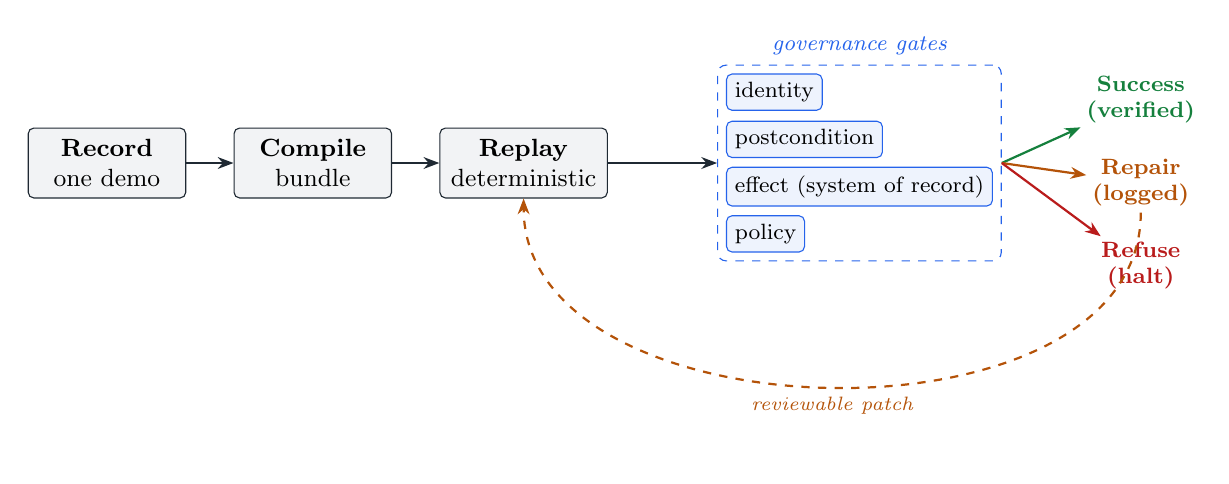
\begin{tikzpicture}[
  font=\small,
  node distance=6mm,
  box/.style={draw=oaink, rounded corners=2pt, align=center, inner sep=4pt,
    minimum height=8mm, fill=white},
  stage/.style={box, fill=oagray!50, minimum width=20mm},
  gate/.style={draw=oablue, rounded corners=2pt, align=center, inner sep=3pt,
    fill=oablue!8, font=\footnotesize},
  outcome/.style={align=center, font=\footnotesize\bfseries, inner sep=2pt},
  flow/.style={-{Stealth[length=2mm]}, draw=oaink, thick},
  ]
  \node[stage] (rec) {\textbf{Record}\\one demo};
  \node[stage, right=of rec] (comp) {\textbf{Compile}\\bundle};
  \node[stage, right=of comp] (rep) {\textbf{Replay}\\deterministic};
  \draw[flow] (rec) -- (comp);
  \draw[flow] (comp) -- (rep);

  % Governance gate stack, to the right of replay (left-aligned so the widest
  % gate does not overrun the Replay node).
  \coordinate (gx) at ($(rep.east)+(15mm,0)$);
  \node[gate, anchor=west] (id)   at ($(gx)+(0,9mm)$)   {identity};
  \node[gate, anchor=west] (post) at ($(gx)+(0,3mm)$)   {postcondition};
  \node[gate, anchor=west] (eff)  at ($(gx)+(0,-3mm)$)  {effect (system of record)};
  \node[gate, anchor=west] (pol)  at ($(gx)+(0,-9mm)$)  {policy};
  \begin{scope}[on background layer]
    \node[draw=oablue, dashed, rounded corners=3pt, fit=(id)(post)(eff)(pol),
      inner sep=3pt, label={[font=\footnotesize\itshape,oablue]above:governance gates}] (gatebox) {};
  \end{scope}
  \draw[flow] (rep) -- (gatebox.west);

  % Three outcomes.
  \node[outcome, right=10mm of gatebox, yshift=8mm, text=oagreen] (ok) {Success\\(verified)};
  \node[outcome, below=3mm of ok, text=oaamber] (heal) {Repair\\(logged)};
  \node[outcome, below=3mm of heal, text=oared] (halt) {Refuse\\(halt)};
  \draw[flow, oagreen] (gatebox.east) -- (ok);
  \draw[flow, oaamber] (gatebox.east) -- (heal);
  \draw[flow, oared] (gatebox.east) -- (halt);

  % Repair feeds back a patch; refusal stops.
  \draw[flow, oaamber, dashed] (heal.south) to[out=-90,in=-90] node[below,font=\scriptsize\itshape]{reviewable patch} (rep.south);
\end{tikzpicture}
\caption{\system{} compiles one demonstration into a deterministic program.
Healthy replay makes no model calls. Each step passes governance gates; the
runtime verifies and succeeds, records a bounded \emph{repair} when a lower-
fidelity rung re-resolves a changed target, or \emph{refuses} when a configured
check cannot be verified. A repair is an auditable patch, never a silent
overwrite of the deployed bundle.}
\label{fig:pipeline}
\end{figure}

\subsection{Record and compile}
A recorder captures actions, frames, element observations, and structural state
when available. Declared secret fields are replaced with runtime parameters.
The compiler emits a bundle containing a workflow program, target crops,
locators, landmarks, postconditions, parameter declarations, and a manifest.
The linear trace is the simplest program; the intermediate representation also
supports states, guarded transitions, branches, loops, and subflows. Given
several demonstrations of the same task, a deterministic multi-trace induction
pass promotes a value that varies at an aligned position to a typed parameter, a
consecutive repeated sub-sequence whose repetition count varies to a loop over an
inferred relation, and a divergence under a detectable condition to a guarded
branch; it makes no model call. Its reach is deliberately narrow and we state
the limit rather than the aspiration: only consecutive repeated bodies are
recognized, so a navigate-away-and-return loop, a paginated loop, and a
per-row-conditional body are not. Where induction cannot certify the shape---an
ambiguous loop around an irreversible action, an undetermined branch condition,
an unhandled zero-result case---it emits an uncertainty and quarantines the
result rather than inventing one, and the compiled workflow stays uncertified
until an operator answers a concrete, grounded question about the specific
divergence.

Parameterization is where a compiler is most tempted to guess, because the
difference between a constant and a parameter is the difference between
replaying a demonstration and running a new case. \system{} therefore infers
parameter \emph{candidates} deterministically---a value typed into a field
carries the field's own label, taken from the recorder's structural capture or,
failing that, from the nearest OCR line left of or above the field rectangle---
and then refuses to apply them. Each candidate is written to a sidecar with the
example value masked, and one batch operator pass confirms, renames, marks
secret, or keeps each as a constant. The default on an unanswered prompt is
\emph{keep constant}: an unconfirmed inference changes nothing, and the bundle
replays exactly as demonstrated. This is deliberate rather than conservative
for its own sake---the parameter name is the identifier an effect contract binds
to and that secrets are keyed by, so naming is confirmed by a human, never
inferred behind the operator's back. The inference makes no model call.

\subsection{Resolution ladder}
For an action target, replay tries evidence in descending order of fidelity:
structured DOM or accessibility identity, local and global template matching,
OCR, landmark geometry, and an optional grounding model. A backend presents a
small common contract for observation and actuation. This provides a pixel
floor without discarding structured evidence on browsers and native desktops.

Healthy execution stops at deterministic tiers and makes zero model calls. A
lower rung resolving a changed but verified target creates a repair patch. The
runtime can save a healed derivative bundle, but does not silently replace the
deployed source bundle.

\begin{figure}[t]
\centering
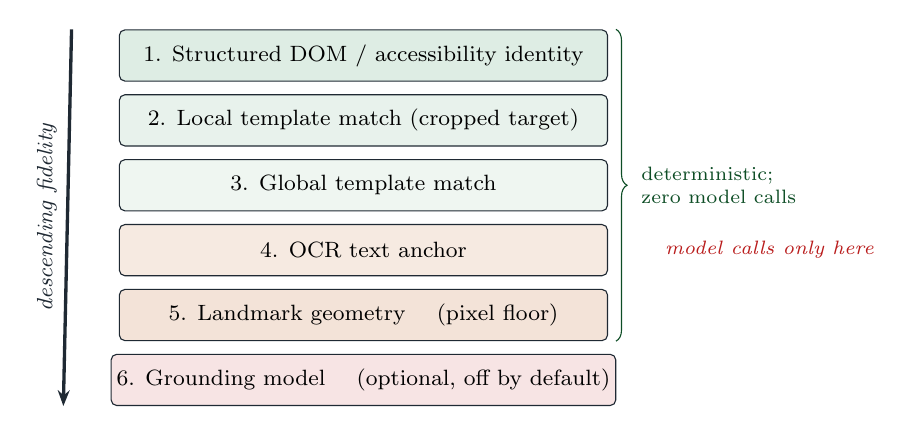
\begin{tikzpicture}[
  font=\footnotesize,
  rung/.style={draw=oaink, rounded corners=2pt, minimum width=62mm,
    minimum height=6.5mm, align=center, inner sep=2pt},
  ]
  \node[rung, fill=oagreen!14] (r1) {1. Structured DOM / accessibility identity};
  \node[rung, fill=oagreen!10, below=1.6mm of r1] (r2) {2. Local template match (cropped target)};
  \node[rung, fill=oagreen!7, below=1.6mm of r2] (r3) {3. Global template match};
  \node[rung, fill=oaamber!12, below=1.6mm of r3] (r4) {4. OCR text anchor};
  \node[rung, fill=oaamber!16, below=1.6mm of r4] (r5) {5. Landmark geometry \quad (pixel floor)};
  \node[rung, fill=oared!12, below=1.6mm of r5] (r6) {6. Grounding model \quad (optional, off by default)};

  \draw[-{Stealth[length=2mm]}, very thick, oaink]
    ($(r1.north west)+(-6mm,0)$) -- ($(r6.south west)+(-6mm,0)$)
    node[midway, rotate=90, anchor=south, font=\footnotesize\itshape]{descending fidelity};

  \node[right=3mm of r3, align=left, font=\scriptsize, text=oagreen!60!black] (det)
    {deterministic;\\zero model calls};
  \draw[decorate, decoration={brace, amplitude=4pt}, oagreen!60!black]
    ($(r1.north east)+(1mm,0)$) -- ($(r5.south east)+(1mm,0)$);
  \node[right=6mm of r4, font=\scriptsize\itshape, text=oared] {model calls only here};
\end{tikzpicture}
\caption{The resolution ladder tries evidence in descending order of fidelity.
Structured identity is preferred; local visual evidence gives a pixel floor for
substrates without a DOM. Rungs 1--5 are deterministic and make no model calls.
A grounding model is an optional last rung, disabled by default, and its rescue
is subject to the same identity and effect checks.}
\label{fig:ladder}
\end{figure}

\subsection{Postconditions and reports}
Each step may carry visual or structural postconditions such as text presence,
region stability, URL change, or window state. Replay writes a human-readable
and machine-readable report with rung, confidence, identity verdict,
postconditions, effects, model calls, elapsed time, repair, and halt reason.
Postconditions are necessary but not sufficient: a success banner is evidence
about the screen, not independent evidence about a database write.

\subsection{Backends and explicit surface selection}
The browser backend is the reference implementation and supplies published
end-to-end evidence against a real third-party application. Windows UI
Automation adds structured candidate enumeration and native actions behind a
typed, authenticated in-session contract. Native macOS binds capture and input
to a unique application window. The RDP and Citrix Workspace backends expose the
same runtime contract over a pixel-only network session. Section~4 reports
scoped task and effect qualifications for the Windows, macOS, and RDP
mechanisms, and a deterministic synthetic stand-in campaign for the Citrix
Workspace backend. A real Citrix ICA/HDX environment is a separate deployment
and inherits neither the RDP qualification nor the stand-in campaign.

The browser is one execution surface among six---\texttt{web},
\texttt{windows}, \texttt{macos}, \texttt{linux}, \texttt{rdp}, and
\texttt{citrix}---and not a privileged default. Each surface fixes an execution
\emph{mode}: \texttt{rdp} and \texttt{citrix} are \emph{external}, driving a
local client window of a remote session through pixels, keyboard, and mouse with
nothing installed inside that session; the others are \emph{in-session}. The
mode is fixed by capability negotiation at qualification and is never silently
switched at run time. Two consequences are enforced at the command line rather
than documented as advice. First, under the production execution profiles a
record or run command that does not name a surface is \emph{refused}, because an
implicit browser default silently decides the substrate a workflow will be
qualified on. Second, a compiled bundle carries the surface it was recorded on,
and running it on a different surface is refused unless the operator passes an
explicit override, which is then recorded in the run report as compatibility
evidence. A cross-surface run is never silent.

\section{Governed Execution}
\label{sec:governance}

\subsection{Identity before action}
Target resolution answers where to act; identity verification asks whether the
resolved target belongs to the intended entity. Structured text is authoritative
where available. On pure-pixel substrates, OCR ambiguity can make distinct
identifiers observationally identical. The safe response is abstention and
halt, not a guessed click. Importantly, identity guarantees apply only to armed
steps. Current real bundles can contain unarmed clicks, so coverage is reported
per workflow and certification policy can impose a minimum.

\subsection{Effect verification}
A screen may paint success after a partial, duplicate, rejected, or stale write.
Consequential steps can therefore declare typed effects and use an independent
verifier against REST, FHIR, or document state. The verifier snapshots the
system of record before and after an action and returns confirmed, refuted, or
indeterminate. A declared effect without a configured verifier halts.

Crucially, the strong-oracle read is performed \emph{out of band}: the verifier
queries the system of record through its own interface (a SQL read on a
read-only role, a REST or FHIR read, or a document or file read), independently
of the substrate that carried the write. It does not parse the pixel stream or
scrape the rendered page. The same effect contract therefore holds whether the
write was driven through a browser DOM, native accessibility, or a pixel-only
remote session: what changes is only the connector, not the check. Because the
read is out of band, an unreachable, unreadable, or unauthenticated system of
record maps to indeterminate and halts; the runtime never upgrades ``I could not
read the record'' into a reported success.

Two consequences follow for pixel-only substrates such as RDP and Citrix. First,
the effect check still applies as long as some out-of-band read path exists: the
RDP qualification in Section~\ref{sec:results}, for instance, reads the persisted
file through guest tools, a channel independent of the RDP display. Second, when
a locked-down session exposes \emph{no} such path, no database, no reachable API,
and no readable file, the transactional strong oracle is simply unavailable. The
only fallback is a same-application re-read of the record, which cannot catch a
partial save, a duplicate, a stale overwrite, or a lost update, and the honest
runtime treats that as a halt rather than a confirmation. On such substrates the
safety guarantee rests instead on the identity gate and halt-on-ambiguity, not on
effect verification. Effects are currently authored per deployment; the compiler
does not infer them from a single demonstration. This is the classic \emph{oracle
problem}
\cite{barr2015oracle} made concrete: the screen is a weak oracle and the
application's own state is the strong oracle (Figure~\ref{fig:oracle}). Many of
the faults it catches---duplicate submission, double delivery, stale
overwrite---are exactly-once and idempotency hazards long studied in
transactional systems \cite{gray1981transaction}. Unlike a general
formal-verification claim, the guarantees here remain scoped to armed steps,
declared effects, configured verifiers, and named policies.

\subsection{The verifier as a pluggable adapter, and its confidence tier}
Because the oracle must be authored per deployment, the interface to it is a
first-class extension point rather than a fixed set of connectors. A verifier
adapter declares a substrate and a confidence tier and implements four
operations: a read-only connection probe, a before-state capture, an
after-state capture, and a verdict. Secrets arrive as environment or
secret-manager \emph{references}, never literals. Shipped adapters cover REST,
GraphQL, FHIR, read-only SQL (with a query whitelist), file and SFTP arrival,
maildir/SMTP delivery, document arrival, and document hashing; a third party
registers its own for a proprietary system of record either programmatically or
by publishing a packaging entry point named for the effect kind it serves. A
plugin that fails to import is a hard error rather than an unknown kind, and a
plugin can never shadow a built-in kind.

Three properties of that interface are load-bearing. First, the adapter result
is deliberately six-valued---confirmed, refuted, unavailable, stale,
conflicting, indeterminate---and only \emph{confirmed} lets a step proceed;
the other five map to a halt, and four of them to an explicit reconciliation
requirement, because ``the record says no'' and ``I could not read the record''
are different facts and must not be collapsed. Second, freshness can only
weaken evidence: a confirmed verdict whose matched record carries a missing,
unparseable, or out-of-window timestamp is demoted to indeterminate, and no
freshness rule can rescue a failure into a pass. Third, each adapter declares
its confidence tier, and a same-screen read-back is explicitly the lowest
tier---a consistency check, never independent system-of-record proof---so a
deployment cannot quietly satisfy an effect requirement with the weak oracle
the mechanism exists to replace. Evidence redaction, likewise, can only
minimize what is retained; it cannot soften a failure into a success.

\subsection{Transaction outcomes, effect journal, and idempotency}
A run's terminal state is not a boolean. \system{} classifies every run into
exactly one \emph{transaction outcome} describing what is known about the
business effect: \textsc{verified}, \textsc{halted-before-effect},
\textsc{reconciliation-required}, \textsc{failed-platform}, \textsc{canceled},
\textsc{rejected-policy}, \textsc{completed-unverified}, and
\textsc{rolled-back}. Only \textsc{verified} is a production success and only
\textsc{verified} is billable; a demonstration-profile completion is
\textsc{completed-unverified} and can never be mistaken for one.
\textsc{halted-before-effect} is reserved for the case where a verifier
affirmatively established that no effect occurred---an unread record is not an
absent record. \textsc{reconciliation-required} therefore dominates every other
non-success bucket: any unresolved delivery uncertainty, any indeterminate
effect verdict, and any refutation that did \emph{not} establish absence lands
there. This is what makes the classification operationally meaningful rather
than cosmetic, because \textsc{reconciliation-required} forbids a blind retry of
the consequential write.

Two records support it. The \emph{effect journal} is a per-step ledger over the
executed consequential steps, recording for each one the digests of the effect
contracts it intended to apply, whether it was actuated and whether delivery was
uncertain, whether the effect was observed present, absent, conflicting, or
unknown, whether independent verification actually ran this run, and how many
reconciliation actions were performed. It is deliberately privacy-safe by
construction: hashes, closed enums, counts, and timestamps only, with no record
values, parameters, or free text, so it can leave the trusted boundary that the
underlying observations cannot. The \emph{idempotency ledger} is an
append-only at-most-once store keyed by a caller-supplied key. A run reserves
its key \emph{before any actuation}, so a crash after the write leaves a
reservation behind; a later run under the same key is refused and recorded
rather than re-actuated. A corrupt ledger fails loud instead of treating keys as
unseen, and the suppressed replay never overwrites the original run's outcome.

\subsection{Governed repair promotion}
Section~\ref{sec:results} reports that the resolution ladder repairs drifted
targets without a model. A repair that could silently become the deployed
program would, however, convert a runtime convenience into an unreviewed change
to a consequential automation. \system{} therefore treats a repair as a
\emph{candidate} and nothing more. A healed or taught bundle is registered as a
candidate record---binding values as digests, failure evidence as hashed
references---and registration failure fails closed by absence: without the
record the healed bundle cannot enter the lifecycle at all.

Promotion runs through an explicit state machine---candidate, reviewed,
replay-passed, fault-passed, approved, staged, canary, active, with rejection
and rollback as terminal states---in which no state may be skipped and no
candidate advances as a side effect of being written to disk. Five gates guard
it. (1) \emph{Contract invariants}: the proposed bundle is diffed against the
prior one across identity, effect, risk, environment, and policy, and any
weakening---a lost identity evidence tier, a lowered quorum, a dropped effect
declaration, a weakened effect tier, a downgraded risk classification, a changed
target application or environment digest, a removed qualification---is refused
unless the bundle carries an explicit new qualification revision. An
incomparable contract is itself a refusal. (2) A \emph{replay campaign} over a
deterministic perturbation battery, which passes only if the binding both
locates the target and verifies its identity in every case. (3) A \emph{fault
campaign} over ambiguity, wrong-entity, stale-target, unexpected-dialog, and
verifier-failure injections, whose pass criterion is inverted: a case passes
only when the binding \emph{refuses}, and an unarmed binding cannot pass at all.
(4) A \emph{human approval} bound to the exact content digests of both bundles,
re-verified against the bundles reloaded from disk, so a later byte change
invalidates it. (5) A \emph{bounded canary} over the first $N$ runs that halts
and reverts the active pointer automatically on the first unverified or silently
incorrect run.

Actors are typed, and the typing is the point: a model may produce a candidate
but may never review, approve, promote, or actuate one, and automation may run
the mechanical campaign and canary steps but may never review or approve. Only
a human actor can move a candidate through review and approval. Rollback is a
single command, restoring a digest-verified copy of the prior bundle that was
staged alongside the proposed one for exactly this purpose. This is why the
runtime can heal aggressively without the healed program becoming the deployed
program: the two are separated by a gate a model cannot open.

\begin{figure}[t]
\centering
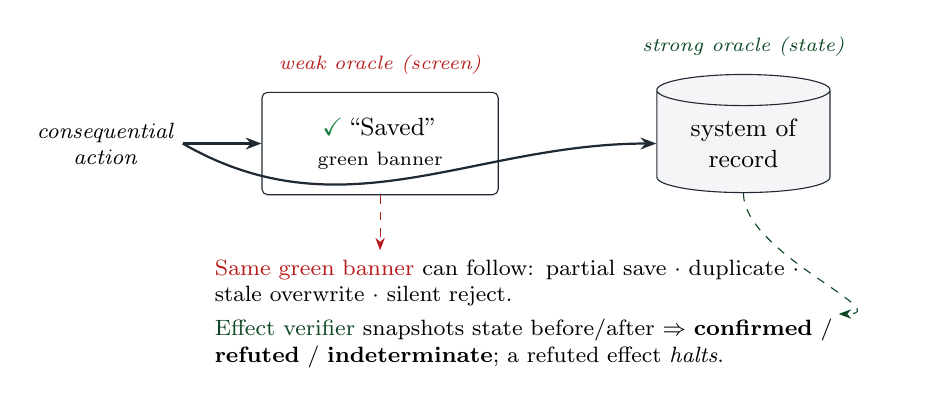
\begin{tikzpicture}[
  font=\small,
  screen/.style={draw=oaink, rounded corners=2pt, minimum width=30mm,
    minimum height=13mm, align=center, fill=white},
  db/.style={draw=oaink, cylinder, shape border rotate=90, aspect=0.28,
    minimum width=22mm, minimum height=15mm, align=center, fill=oagray!40,
    inner sep=1pt},
  verdict/.style={align=left, font=\footnotesize},
  ]
  % The action.
  \node[align=center, font=\footnotesize\itshape] (act) {consequential\\action};
  \node[screen, right=10mm of act] (scr)
    {\textcolor{oagreen}{$\checkmark$}\,``Saved''\\\scriptsize green banner};
  \node[db, right=20mm of scr] (db) {system of\\record};

  \draw[-{Stealth[length=2mm]}, thick, oaink] (act) -- (scr);
  \draw[-{Stealth[length=2mm]}, thick, oaink] (act.east) to[out=-30,in=180] (db.west);

  % Weak vs strong oracle labels.
  \node[above=1mm of scr, font=\scriptsize\itshape, text=oared] {weak oracle (screen)};
  \node[above=1mm of db, font=\scriptsize\itshape, text=oagreen!55!black] {strong oracle (state)};

  % The disagreement.
  \node[verdict, below=7mm of scr, text width=78mm, xshift=18mm] (gap)
    {\textcolor{oared}{Same green banner} can follow: partial save $\cdot$
     duplicate $\cdot$ stale overwrite $\cdot$ silent reject.
     \\[1mm]
     \textcolor{oagreen!55!black}{Effect verifier} snapshots state before/after
     $\Rightarrow$ \textbf{confirmed} / \textbf{refuted} / \textbf{indeterminate};
     a refuted effect \emph{halts}.};
  \draw[-{Stealth[length=1.6mm]}, oared, dashed] (scr.south) -- (gap.north -| scr.south);
  \draw[-{Stealth[length=1.6mm]}, oagreen!55!black, dashed] (db.south) to[out=-90,in=0] (gap.east);
\end{tikzpicture}
\caption{Effect verification separates the weak screen oracle from the strong
system-of-record oracle. A rendered success is evidence about pixels, not about
a persisted write; only an independent before/after snapshot of the application's
state can refute a silent wrong action. In the end-to-end fault study this
reduced silent acceptance from 54 of 90 runs to 9 of 90 under a single
out-of-band record oracle, and to 0 of 90 only once the read path covered every
mutable surface the action could touch.}
\label{fig:oracle}
\end{figure}

\subsection{Policy and refusal}
The linter exposes unarmed clicks, vacuous postconditions, and risk-classifier
gaps. Certification evaluates a named policy before deployment. A strict run
gate can require certification, identity and effect coverage, encryption, and
manifest integrity. Passing a policy means only that its assertions hold; it is
not a general safety proof.

\subsection{Sanitized artifact derivatives}
Compilation is not de-identification. When an artifact crosses a boundary, the
launch protocol inventories the source, transforms a copy with type-specific
handlers, rescans the derivative, records unresolved findings and tool versions,
and binds local review to the derivative hash. Unknown or unresolved content is
refused. Sanitized authoring evidence is distinct from runtime observations:
opening a live patient record can reintroduce protected information, which must
remain inside the declared trusted execution boundary.

\section{Evaluation Methodology}
\label{sec:method}

We separate comparative task performance, breadth, transactional safety, and
identity availability. A single aggregate success rate would hide materially
different errors.

\paragraph{Comparative conditions.}
Both repeated-workflow comparisons were generated on 2026-07-08 on the recorded
platform \texttt{macOS-15.7.3-arm64-arm-64bit}. The compiled and agent arms
drove the same vision-only Playwright backend: screenshots in and pixel clicks,
typed text, key presses, and scrolling out, with no DOM selectors at runtime.
The agent condition used \texttt{claude-sonnet-5} with the
\texttt{computer\_20251124} tool and
\texttt{computer-use-2025-11-24} beta header. Agent costs are calculated from
recorded token usage and the list-price schedule stored in each raw result; the
compiled condition recorded no model calls. The agent is a single-attempt
observe-act loop given the task goal and the same settled screenshots the
replayer uses, without a system prompt, planning or reflection scaffolding, or
whole-task retry, and bounded by per-run action and cost caps. It is a
same-backend reference rather than a maximally scaffolded agent. The measured
latency and cost differences characterize only these exact configurations; they
do not predict what additional planning, reflection, or retry scaffolding would
cost or recover, and they are not a reliability comparison.

\paragraph{Outcome taxonomy.}
Success means the external task oracle is satisfied. A safe halt stops without
the intended effect. Over-halt is a safe halt when the intended correct action
was in fact available. Silent incorrect success means the runtime reports
success while the external oracle disagrees. False abort means the intended
effect occurred but the runtime reports failure.

\paragraph{Scripted coverage counts, not sampled rates.}
The fault-injection and end-to-end studies use localhost, make no model calls,
and inject a fixed fault at the persistence boundary. In the released matrices,
the repeated outcomes were invariant within each arm--scenario cell. Those
repeats confirm reproducibility in this implementation and environment; they are
not independent samples from a target population. We therefore report run
counts as a \emph{coverage matrix} over a small, hand-authored fault taxonomy,
not as an estimate of a production incidence rate. Inferential confidence
intervals would require a sampling design and a target distribution that this
study does not have. Two consequences are load-bearing for how these numbers
should be read. First, the screen-versus-effect headline is determined by the
authored differentiating classes, and the out-of-band-versus-complete-read-path
gap rests on exactly one class, rather than on a sampled workload distribution.
Second, the taxonomy is an adversarial transactional-fault lineage
\cite{gray1981transaction} chosen to differentiate oracles; it is not weighted
to any measured EMR or lending incident distribution, so a figure such as the
screen arm's 60\% is fault coverage under this taxonomy, never an expected
production frequency.

\paragraph{OpenEMR comparison.}
The task logs into the shared public OpenEMR demonstration site, searches a
patient, opens Patient Messages, adds a parameterized note, and saves. The
compiled arm has 20 runs and the computer-use-agent arm 10. Both use the same
task-level success check. The shared public instance is mutable and the study is
not fully reproducible in CI; it is field evidence, not a production study.

\paragraph{MockMed comparison.}
The bundled browser fixture performs a triage workflow. The compiled arm has
100 runs and the agent arm 20. This is the CI-reproducible anchor, but the
application is purpose-built and is not evidence about hostile enterprise UIs.

\paragraph{Public-web reliability corpus.}
Twenty-nine public, unauthenticated applications are recorded, compiled, and
replayed once on an unchanged UI using an external goal oracle. This study is
descriptive: one run per application does not meet the repeated-trial standard
for a capability claim, and the selection excludes SSO-walled and desktop
targets.

\paragraph{Transactional fault model (perception included, screen arm only).}
Seven persistence faults and controls are injected at a real HTTP persistence
boundary behind the MockMed UI, with 10 repeats per class. Database state, not
the UI report, is the oracle. This study is the one that exercises the full
perception path---a real browser, real screenshots, and real OCR through the
resolution ladder---but it measures only the screen-only arm; it carries no
effect-verified arm and contributes no effect-verified number to this paper. It
is complementary to, and separate from, the end-to-end study below.

\paragraph{End-to-end effect verification (governed path, perception stubbed).}
The headline safety result is measured through the actual governed replay path,
not an in-process stub. Ten persistence scenarios, seven fault classes plus an
accepted-write control and two delivery controls, are each run nine times per
arm. Every write is issued by the replayer's actuator as an HTTP POST to an
on-disk SQLite system of record. We state the boundary of ``end to end''
precisely, because it is the obvious thing to overclaim: what is real here is
the governed decision path---the replayer, its actuation tier, its effect
verifier, the policy gates, and the transaction-outcome classification---while
the observation backend and vision stack are null stubs, so this study measures
\emph{verification and refusal}, not GUI perception. Perception is covered by
the browser-and-OCR fault-model study above, whose arm is screen-only. No single
released study covers both at once, and we do not report one as though it did.
Each trial contains three operationally
distinct paths: the actuator writes over HTTP; the system-under-test effect
verifier reads through a separate REST endpoint and connection; and the
benchmark ground truth opens the SQLite file read-only over every table,
fingerprints canonical typed schema and row content, and classifies the
before/after state without seeing the write's success flag. The verifier and
judge necessarily observe the same persisted system of record, but they share
neither a read channel nor classifier implementation, so the system-under-test
verifier cannot define its own score. This is operational independence, not
independence of the business specification. We evaluate three arms:
screen-only banner verification, an out-of-band effect oracle whose read path
covers the record surface, and a complete effect oracle whose read path covers
every mutable surface the action can touch. This supersedes an earlier in-process
study in which the effect verifier and the ground truth read the same object,
which made its zero circular by construction. Zero model calls, localhost only.

\paragraph{Second domain: lending.}
To test generalization beyond healthcare, the same effect-verification protocol
is replicated on MockLoan, a loan-disbursement authorization workflow with its
own SQLite ledger. Twelve tasks span the seven EffectBench divergence categories,
a lending-local cross-surface collateral variant of the extra-write category,
and clean and idempotent controls. Each runs three times per arm. The product
arms read their declared surface through REST; the benchmark judge instead opens
the persisted SQLite file through a separate read-only connection before and
after each write, discovers business tables from SQLite's catalog, and
uses benchmark-local canonical typed row and table-content classification rather
than the runtime effect classifier. One task funds a decoy loan; post-action,
identity-sensitive readback locates the trial-unique persisted row by memo and
product, then verifies its loan identifier against the intended loan. Zero model
calls.

\paragraph{Multi-application workflows.}
The studies above are single-application, linear, worklist-driven form fills of
roughly five to fifteen recorded steps, which is a fair criticism of the suite's
complexity. Two benchmarks were added to close that gap. \emph{AP invoice} is an
accounts-payable intake spanning a maildir inbox, a PDF document, an ERP
three-way match, a payments API, an exception queue, and an outbound mail
gateway: two applications, five modalities, 32 executed action steps over a
five-row worklist, with branching on match route and discount eligibility.
\emph{O2C reconciliation} is an order-to-cash billing reconciliation spanning an
exported CSV worklist, a comparison pass, ledger adjustments through a UI-only
gateway with no adjustment API, reconcile marks over REST, and a results
spreadsheet written back and re-read from disk across two separate SQLite
systems of record: 26 executed action steps over a ten-row worklist. Each
benchmark runs five scenarios---one healthy and four exception paths---three
times in each of two arms. The \emph{naive} arm runs the demonstration profile
and trusts the application's own banner; the \emph{governed} arm runs the
production profile under a named policy that requires system effects for every
write and prohibits unconfirmed effect bindings. A benchmark-local ground truth
reads both databases directly and audits per-table deltas. Both fixtures are
synthetic and localhost-only, every consequential action is actuated through the
replayer's API tier, and no model is called; as with the end-to-end study,
these measure governed workflow semantics and cross-system effects, not GUI
perception and not document understanding.

\paragraph{Citrix ICA/HDX: a deterministic stand-in, not Citrix.}
No real Citrix ICA/HDX result is reported in this paper. What is reported is a
qualification of the shipping Citrix Workspace backend---unmodified---against a
deterministic synthetic stand-in in which only the backend's window-client seam
is replaced by an in-process source of synthetic frames that the real backend
decodes, hashes, and DPI-maps. Sixteen ICA/HDX-class conditions (session launch
and readiness, lock and unlock, reconnect and roaming, minimize, occlusion, move
and resize, single and multi-monitor geometry, DPI and scaling, compression and
codec artifacts, latency and delayed frames, keyboard layout and IME, clipboard
restriction, focus theft, unexpected dialogs, uncertain submission, and
out-of-band persisted-state readback) are exercised over 29 trials, with an
out-of-band in-process oracle and never the on-screen banner. This exercises no
HDX codec, no ICA compression, and no Workspace-client transport; the released
artifact records \texttt{is\_real\_ica\_hdx: false} and
\texttt{ica\_hdx\_accepted: false}, and its status manifest reports
real-protocol environment evidence as \texttt{pending}. We treat it as evidence
about the backend's gating logic under adverse remote-display conditions, and as
nothing else.

\paragraph{Released benchmark.}
The metric and fault taxonomy are packaged as EffectBench, a standalone,
versioned, and independently runnable benchmark (specification version 1.0.0), so
that the silent-wrong-effect rate can be measured against any GUI or API
automation, not only ours. We state its current scope honestly, because the
reusable surface a third party can run is narrower than the specification.

\emph{What is public.} The MIT synthetic sample is one fixture, the MockMed
anchor, and it covers five of the seven divergence categories (C1--C5) plus
controls, on the \texttt{web} substrate alone. C6 (homonym) and C7
(no-op/wrong-target) are specified but exercised only by the container-gated
real-system-of-record packs and the private hardened corpus, as are the desktop
and remote-display substrates. The differentiating cases are therefore defined in
the open and measured behind a gate. A submission may target any subset it can
reach and must report which pack and split it ran.

\emph{What the public pack hands away.} The reference pack ships the synthetic
system of record together with its reference oracle. In a real deployment,
authoring a cheap, correct, independent oracle for a legacy system of record is
the whole cost, and this paper does not claim to remove it: effects are authored
per deployment and the compiler does not infer them
(Section~\ref{sec:governance}). A benchmark that supplies the oracle therefore
measures whether a system uses one, not whether it could obtain one. We mark the
built-in oracle reference-only rather than expose it to the system under test as
a general capability, and a pluggable interface lets a third party bring its own
system of record and its own independent oracle. That is the honest boundary of
what the public pack tests.

\emph{What is not yet demonstrated.} The two baselines scored so far are our own
screen-only and effect-verified arms, so fair cross-system ranking is a design
property rather than a shown one. The public fixture is also small, fixed, and
open, which is exactly the shape a submission can special-case; the private
hardened corpus is the intended mitigation, but a non-gameability argument that
rests on a corpus the reader cannot inspect is asserted rather than
demonstrated. Both gaps close only when an independent system of record and an
independently scored third-party submission enter the public pack.

\paragraph{Identity ladder.}
Adversarial same-name/same-date-of-birth homonyms differ by confusable glyphs
such as O/0 and l/1. The actual replayer stack is evaluated with structured and
pure-pixel configurations. False accept and over-halt are both reported because
a system can obtain zero wrong clicks by refusing every correct one.

\paragraph{Desktop and remote-substrate qualification.}
These mechanism studies are task-bound rather than comparative. Windows UIA is
evaluated on one in-tree WinForms Patient Notes workflow in a Windows 11 ARM VM.
Each counted trial starts from a clean snapshot, writes a trial-unique note, and
uses an independent SQLite query as the effect oracle; stale and ambiguous
candidate controls must leave every row unchanged. Native macOS is evaluated on
one macOS 15.7.3 arm64 host using TextEdit, exact file-byte readback, and a
two-window ambiguity control. The preserved batch report classifies graceful-
close cleanup warnings as failure; a separate hash-bound offline adjudication
accepts only the three action effects and ambiguity refusal after verifying the
exact harness processes and temporary root were absent. RDP is evaluated over
Aardwolf 0.2.14 into one 1280x800 Parallels Windows 11 snapshot: input through
the Windows Run dialog creates a trial-unique file whose exact contents are read
back through guest tools independently of the RDP channel. Each promoted task
has three counted trials, records model calls, silent incorrect success and
over-halt, and retains environment-cleanup evidence.

\section{Results}
\label{sec:results}

\paragraph{Headline: an independent effect check catches silent wrong actions
that the screen misses, and only as far as it can read.} The paper's central
claim is a safety one, and we measure it through the live replayer's governed
actuation and verification path, with the observation backend and vision stack
stubbed (Section~\ref{sec:method}).
Ten persistence scenarios, seven fault classes plus an accepted-write control and
two delivery controls, are each driven nine times per arm through the real
governed path: the replayer's actuator writes over HTTP, the system-under-test
verifier reads through REST, and the benchmark judge reads SQLite directly with
separate classifier code. Judged by the \emph{screen},
the same signal an agent
or a script trusts, replay silently accepted a wrong persisted effect on 54 of 90
fault runs (60\%). An out-of-band effect verifier that reads the record back over
a different endpoint than the write drove silent acceptance down to 9 of 90
(10\%). Extending that verifier to a complete system-of-record read path, one
that covers every mutable surface the action can touch, drove it to 0 of 90
(Figure~\ref{fig:silentbar}). The residual 9 of 90 is the honest mechanism
finding: they are a single fault class, a collateral write to a billing surface
the out-of-band oracle's read path never covered, so the guarantee is exactly as
strong as the oracle's read coverage. False aborts are a constant 9 of 90 in all
three arms, a conservative halt on a commit whose outcome is unknown to the
client, so they do not distinguish the oracles. This end-to-end measurement
supersedes an earlier in-process fault study whose effect and ground-truth checks
read the same object, which made its zero circular by construction; the numbers
here come from the real replayer with operationally separate write, read-back,
and ground-truth paths. These paths do not make the shared business
specification independent; Section~\ref{sec:limits} bounds that closed-world
assumption.

\paragraph{Per scenario, the gap is driven by six differentiating classes and
closed by one read-path extension.} Table~\ref{tab:e2eclasses} decomposes the
same 90 runs per arm. Six of the ten scenarios differentiate the screen from an
out-of-band record oracle; exactly one, the collateral write, differentiates the
single-surface oracle from a complete read path. Three scenarios---optimistic
rendering followed by rejection, session loss, and a timeout after a successful
commit---halt in every arm, so they carry no oracle signal at all; the last of
these is the constant false abort. Read the table as a coverage matrix over
hand-authored classes, not as a distribution: the headline is a property of
which classes were authored.

\begin{table}[t]
\centering
\caption{End-to-end fault study, per scenario, nine runs per cell. ``Slip''
means the arm reported success while the independent ground truth found a wrong
persisted effect; ``halt'' means the arm refused. The screen arm slips on six
classes, the single out-of-band oracle on one, and the complete read path on
none. Rows marked ``halt'' in all three arms carry no oracle signal.}
\label{tab:e2eclasses}
\small
\begin{tabular}{llccc}
\toprule
Scenario & Ground-truth effect & Screen & Out-of-band & Complete read \\
\midrule
Clean write (control)    & correct          & pass & pass & pass \\
No persistence           & absent           & slip & halt & halt \\
Partial save             & partial          & slip & halt & halt \\
Duplicate submission     & duplicate        & slip & halt & halt \\
Wrong record             & wrong record     & slip & halt & halt \\
Stale overwrite          & collateral loss  & slip & halt & halt \\
Collateral write         & collateral write & slip & slip & halt \\
Optimistic then reject   & absent           & halt & halt & halt \\
Session loss             & absent           & halt & halt & halt \\
Timeout after commit     & correct          & halt & halt & halt \\
\bottomrule
\end{tabular}
\end{table}

\paragraph{With real perception, the screen misses five of seven fault types.}
The study above stubs the vision stack. A separate transactional study at the
same persistence boundary keeps perception real---a live browser, real
screenshots, and OCR through the resolution ladder---and injects the same class
of faults. There, screen-only
verification silently mishandled five of seven injected fault classes: partial
save, duplicate submission, optimistic UI followed by rejection, stale overwrite,
and double delivery. There were 10 consistent repeats per class. That study
carries no effect-verified arm, so it establishes the screen-oracle failure
under real perception and nothing about the fix; the fix is measured only in the
stubbed-perception study above. We report the pair rather than a single number
because no released study covers both perception and effect verification at
once. The improvement itself has two non-optional
preconditions in either case: the effect must be authored and the verifier
deployed.

\paragraph{Generalization: the same silent-wrong ladder on a second,
non-healthcare domain.} The effect-verification result is not specific to
clinical records, and it reproduces the healthcare three-arm ladder rather than
an easier two-arm version. On MockLoan, a loan-disbursement authorization
workflow with its own ledger and a second, collateral fee surface, screen-only
verification silently accepted 24 of 36 wrong ledger effects (67\%) while
over-halting none. A single out-of-band oracle over one surface left 3 of 36,
exactly the collateral-write residual the healthcare study exhibits: a spurious
fee posts to a surface the disbursement oracle does not read. Extending to a
complete read path drove it to 0 of 36, with 3 of 36 over-halts.
That final arm also classified 18 of 36 runs as wrong actions: the verifier
detected an incorrect effect after persistence and refused to certify it. Thus
zero SWER means zero \emph{silently accepted} wrong effects in this matrix, not
rollback, prevention, or zero incorrect writes.
Broken out by class, screen-only verification again silently mishandled the same
2xx-but-wrong fault classes. In the decoy-loan task, post-action readback finds
the trial-unique wrong-loan row and both effect arms report a detected wrong
action rather than an over-halt. This is the same mechanism, and the same read-coverage
residual, as the healthcare study, on a different system of record; both
applications are synthetic and built by the same authors, so the replication
shows the pattern transfers across two record shapes we designed, not that it
transfers to a hostile production system.

\begin{figure}[t]
\centering
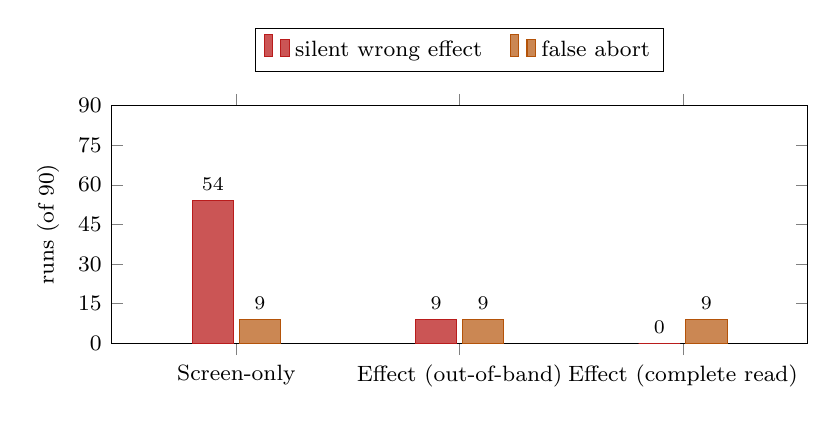
\begin{tikzpicture}
\begin{axis}[
  ybar,
  bar width=15pt,
  width=0.86\linewidth,
  height=4.6cm,
  ymin=0, ymax=90,
  ylabel={runs (of 90)},
  ylabel style={font=\footnotesize},
  symbolic x coords={Screen-only, {Effect (out-of-band)}, {Effect (complete read)}},
  xtick=data,
  xticklabel style={font=\footnotesize},
  ytick={0,15,30,45,60,75,90},
  yticklabel style={font=\footnotesize},
  enlarge x limits=0.28,
  legend style={font=\footnotesize, at={(0.5,1.14)}, anchor=south,
    legend columns=-1, /tikz/every even column/.append style={column sep=8pt}},
  nodes near coords, nodes near coords style={font=\scriptsize},
]
\addplot[fill=oared!75, draw=oared] coordinates {(Screen-only,54) ({Effect (out-of-band)},9) ({Effect (complete read)},0)};
\addplot[fill=oaamber!70, draw=oaamber] coordinates {(Screen-only,9) ({Effect (out-of-band)},9) ({Effect (complete read)},9)};
\legend{silent wrong effect, false abort}
\end{axis}
\end{tikzpicture}
\caption{Same 90 injected-fault runs, three verification policies, measured
through the live replayer's governed actuation and verification path (with a
null observation backend and vision stack) and judged by an independent ground
truth.
Screen-only verification silently accepted 54 wrong persisted effects; an
out-of-band effect oracle that reads the record back cut that to 9 (one
uncovered collateral-write class); a complete system-of-record read path drove it
to 0. False aborts are a constant 9, a safe halt on an unknown-outcome commit.
This is the failure mode general computer-use agents and selector RPA do not
measure.}
\label{fig:silentbar}
\end{figure}

\paragraph{Complexity: the same result holds on branching, multi-application
workflows.} A fair objection to everything above is that the workflows are
short, linear, single-application form fills. Two multi-application benchmarks
answer it directly (Section~\ref{sec:method}). Across both, 30 governed runs
produced zero silent incorrect successes and zero healthy-path over-halts, while
the same 30 runs under the naive banner oracle produced 6 silent incorrect
successes. Every healthy governed run classified \textsc{verified} under the
transaction taxonomy; no naive run did, because the naive arm never obtains
independent effect evidence and therefore terminates
\textsc{completed-unverified} even when it is right. Zero model calls throughout.

Table~\ref{tab:multiapp} shows why the taxonomy matters more than a success
rate. In the AP-invoice collateral-approval scenario the naive arm reports
success three times over while an adjacent record is overwritten; the governed
arm reports \textsc{reconciliation-required} and catches it on all three. In the
payment-confirmation outage both arms fail to confirm, but only the governed arm
says so, and in both arms the duplicate-attempt check confirms that a retry
under the same idempotency key is refused rather than re-actuated. In the O2C
phantom write-back the results spreadsheet returns HTTP 200 with a banner and
persists nothing; re-reading the file catches it three times out of three. These
are deterministic synthetic fixtures with hand-authored exception paths, three
runs per cell, and API-tier actuation, so they are a coverage matrix over
workflow shapes---not an incidence rate and not evidence about perception.

\begin{table}[t]
\centering
\caption{Multi-application workflows, three runs per scenario per arm
(30 governed and 30 naive runs total). Cells give the transaction outcome, which
was invariant across the three repeats. V = \textsc{verified},
CU = \textsc{completed-unverified}, H = \textsc{halted-before-effect},
R = \textsc{reconciliation-required}. Starred cells are the ones the naive
banner oracle silently accepts.}
\label{tab:multiapp}
\small
\begin{tabular}{lllcc}
\toprule
Benchmark & Scenario & Fault & Naive & Governed \\
\midrule
AP invoice & healthy               & ---                  & CU  & V \\
AP invoice & missing PO            & precondition absent  & H   & H \\
AP invoice & duplicate invoice     & ambiguous duplicate  & H   & H \\
AP invoice & collateral approve    & adjacent overwrite   & CU* & R \\
AP invoice & payment outage        & uncertain delivery   & CU  & R \\
O2C recon  & healthy               & ---                  & CU  & V \\
O2C recon  & missing in ledger     & precondition absent  & H   & H \\
O2C recon  & ambiguous duplicate   & ambiguous target     & H   & H \\
O2C recon  & stale snapshot        & optimistic concurrency & H & H \\
O2C recon  & phantom write-back    & 200 without persist  & CU* & H \\
\bottomrule
\end{tabular}
\end{table}

\paragraph{Compiled replay removes per-run reasoning on demonstrated tasks.}
Table~\ref{tab:comparison} shows that, on these two already-demonstrated tasks,
compiled replay completed every measured run with lower median latency and no
model calls. The unequal, small samples do not establish superior reliability.
The correct inference is narrower: repeated reasoning was unnecessary for the
healthy executions measured here.

\begin{table}[t]
\centering
\caption{Bounded repeated-workflow comparison. Model API costs are estimates
derived from recorded token usage and artifact-declared list prices; they
exclude authoring and operations.}
\label{tab:comparison}
\begin{tabular}{llrrrr}
\toprule
Task & Arm & Success & $n$ & Median (s) & Model cost/run \\
\midrule
OpenEMR & Compiled & 20/20 & 20 & 39.2 & \$0.00 \\
OpenEMR & Agent & 10/10 & 10 & 70.4 & \$0.55 \\
MockMed & Compiled & 100/100 & 100 & 4.9 & \$0.00 \\
MockMed & Agent & 20/20 & 20 & 37.5 & \$0.27 \\
\bottomrule
\end{tabular}
\end{table}

\paragraph{Repair under drift: the compiler heals what breaks the agent's day.}
The comparison above is the healthy path. To exercise the ``govern every
repair'' half of the thesis, we forced the MockMed interface to re-render with a
dark palette, invalidating every recorded template crop. As a single observation
per arm, compiled replay self-healed in 9.7\,s with 8 target repairs and zero
model calls, while the same computer-use agent under the same drift took 87.4\,s
and \$0.63 across 24 model calls. One run is not a reliability claim, but it
shows the mechanism working end to end: the resolution ladder re-resolved changed
targets deterministically and logged each as a reviewable patch rather than
re-reasoning the whole task.

\paragraph{Breadth: weak postconditions can still emit a green report.}
On the one-run public-web corpus, all 29 recordings compiled; 17 replays reached
a verified success, 10 halted safely, and 2 reported success while the external
oracle disagreed. Both silent wrong actions were vacuous successes under an
environment blocker rather than a harmful persisted write, but they demonstrate
that weak postconditions can still yield a green report. Because each app ran
once and the corpus excludes authenticated enterprise and desktop applications,
these counts are failure discovery, not a generalization rate estimate.

\paragraph{Identity: zero false accepts, honestly at the cost of availability.}
The integrated identity ladder recorded zero false accepts in every tested
configuration. Structured browser identity also had zero over-halts on 14
correct homonym cases. Pure-pixel configurations halted on all correct
confusable cases: zero false accepts at 100\% over-halt. This is the intended
safety/availability disclosure, not evidence that pixel-only identity is ready
for dense clinical lists.

\paragraph{Substrate reach: one named task per substrate, not a support claim.}
The governed contract is not browser-specific, but the evidence for that is
three named tasks, not three platforms. Table~\ref{tab:substrates}
qualifies three additional substrates on one named task and environment each,
with an independent effect oracle and refusal controls. Nothing here licenses a
claim about arbitrary applications on those platforms.

\begin{table}[t]
\centering
\caption{Scoped substrate qualifications. Each row is one named task and
environment, not an arbitrary-application support claim.}
\label{tab:substrates}
\begin{tabular}{llll}
\toprule
Substrate & Effect trials & Refusal controls & Independent oracle \\
\midrule
Windows UIA & 3/3 & stale 3/3; ambiguous 3/3 & SQLite row state \\
Native macOS & 3/3 & ambiguous 1/1 & exact file bytes \\
Network RDP & 3/3 & readiness/timeout gate & guest-tools file readback \\
\bottomrule
\end{tabular}
\end{table}

The Windows UIA counted matrix recorded 12 native structural-action receipts,
three independently confirmed note effects, three stale-target refusals, three
ambiguous-target refusals, zero silent incorrect successes, zero over-halts, and
zero model calls. The native receipts establish delivery to a unique refreshed
fingerprint; the SQLite oracle establishes the business effect.

On macOS, all three isolated TextEdit replace-and-save trials matched the exact
expected file bytes, and the two-window control refused without changing either
file. There were zero silent incorrect successes and zero over-halts. We retain
the original failed batch classification and use its separate adjudication only
for these action-effect and refusal observations.

The network RDP batch completed three of three Windows Run-dialog unique-file
tasks with exact guest-tools readback. Trial latencies were 51.845, 10.467, and
7.477 seconds, with zero failures, zero silent incorrect successes, zero
over-halts, and zero model calls. Snapshot cleanup restored the pre-run inventory
and suspended base state. Together these studies qualify the named substrate
mechanisms; they do not transfer to other applications, environments, or Citrix.

\paragraph{Citrix: the backend passes a deterministic stand-in, which is not
Citrix.} We report one result about Citrix and it is deliberately a negative
claim wrapped around a positive one. The shipping Citrix Workspace backend,
unmodified, was exercised over 16 ICA/HDX-class conditions in 29 trials against
a deterministic synthetic stand-in, with only its window-client seam replaced.
All 29 trials met their expectation, with zero silent incorrect successes, zero
silent writes, zero healthy-path over-halts, and zero model calls; the two
banner-bearing trials are the informative ones, since one confirms a persisted
effect only through the out-of-band oracle and the other refuses a green banner
that no independent record supports. This is evidence that the backend's
fresh-frame, focus, DPI, identity, readiness, one-shot-actuation, and
effect-verification gates behave correctly under adverse remote-display
conditions. It is \emph{not} evidence about Citrix. No HDX codec, ICA
compression, or Workspace-client transport was exercised; the frames are
synthetic and the oracle is in-process. The released artifact records
\texttt{is\_real\_ica\_hdx: false} and \texttt{ica\_hdx\_accepted: false}, and
its status manifest reports real-protocol environment evidence as
\texttt{pending}. Any statement that \system{} ``runs on Citrix'' would be
unsupported by this paper.

\section{Limitations and Threats to Validity}
\label{sec:limits}

The single largest limitation is stated first and without hedging: \emph{no
external organization has deployed this system}. Every result in this paper was
produced by its authors, on synthetic fixtures or a shared public demonstration
instance, in a controlled environment. There are zero external pilots, zero
production workloads, and therefore zero field-reliability evidence of any kind.
Nothing in this paper should be read as a claim about how the system behaves in
someone else's hands.

The evidence does not establish long-term reliability, maintenance effort,
total cost of ownership, multi-tenant scale, or safety in clinical production.
OpenEMR uses a shared public demonstration site and a small sample. MockMed is a
fixture, and the second-domain lending study is likewise a bounded mechanism
study (twelve tasks, three trials each) on a purpose-built MockLoan ledger, not a
production lending system. The two multi-application benchmarks add branching
and cross-system effects but are equally synthetic, localhost-only, and
hand-authored, with three runs per cell. The breadth corpus has one trial per
application and selection bias toward public no-auth browser apps. No published
study covers weeks of natural drift or a representative distribution of customer
workflows.

Two evaluation paths are measured separately and neither covers the other. The
end-to-end effect study, the lending study, and the two multi-application
benchmarks all actuate through the replayer's API tier with a null observation
backend and a null vision stack, so they measure governed decision, verification,
refusal, and transaction classification---not GUI perception, and not document
understanding. The browser-and-OCR fault study and the public-web breadth corpus
exercise perception, but the fault study carries only a screen-only arm. A study
that exercises real perception \emph{and} effect verification on the same runs
does not yet exist, and no number in this paper should be read as though one
did.

Identity is only checked on armed steps. Risk classification uses keywords and
can miss an icon-only or indirect write. Visual postconditions do not verify a
system-of-record effect. Effect declarations and verifiers require deployment
work. Optional model rescue can false-rescue an ambiguous state, and measured
grounding is weak on dense lists. Human review can catch contextual sanitation
errors but is not proof of de-identification.

Several mechanisms described in Section~\ref{sec:governance} are presented as
mechanisms and are not the subject of a reported measurement. The
transaction-outcome taxonomy is exercised by the multi-application benchmarks,
where it distinguishes \textsc{verified}, \textsc{halted-before-effect}, and
\textsc{reconciliation-required} on hand-authored exception paths, and the
idempotency ledger is exercised by the duplicate-attempt checks in those runs;
but the verifier plugin seam, the governed repair promotion lifecycle, and
explicit surface selection are described from their implementations and their
unit-level contracts, with no benchmark that quantifies, for example, how often
a contract-invariant check correctly refuses a real drifted bundle or how much
operator time promotion costs. Describing a governance mechanism is not
evidence that it holds up under an adversarial operator or at fleet scale.

The substrate qualifications cover one Windows UIA workflow and VM snapshot,
one macOS host and TextEdit task, and one RDP task and snapshot. They establish
working observation, actuation, refusal, and effect-oracle mechanisms in those
environments, not reliability across application families or deployment fleets.
Remote display introduces compression, scaling, latency, coordinate,
lock-screen, credential, input-acceptance, and identity-availability variables.
No measured result covers real Citrix ICA/HDX, so RDP evidence does not transfer
to a Citrix deployment. The Citrix campaign reported in
Section~\ref{sec:results} is a \emph{deterministic synthetic stand-in}: the
shipping backend is real and unmodified, but its window-client seam is replaced
by in-process synthetic frames, so no HDX codec, ICA compression, or
Workspace-client transport is exercised and the effect oracle is an in-process
store. Its degradation conditions are image transforms, not a Thinwire
bitstream. It is evidence about the backend's gating logic under adverse
remote-display conditions and about nothing else; the released artifact and its
status manifest say so in machine-readable form. Citrix is a pixel-only
remote-display environment in the same
class as the measured RDP backend, and the resolution ladder and identity gate
are substrate-independent by construction, but the paper reports no
real-protocol ICA/HDX
measurement. A concrete validation would record and compile a workflow inside a
real Citrix Workspace session, replay it through the vision-only rungs of the
ladder over the ICA/HDX channel, and confirm the identity gate refuses ambiguous
targets and that an out-of-band effect oracle catches an injected transactional
fault. That study is not reported here.

Effect verification also has a substrate-dependent reach that the RDP row can
obscure. The strong oracle is only available when the system of record can be
read out of band, through a database, API, or file interface independent of the
substrate that carried the write. The RDP qualification reads the persisted file
through guest tools, an out-of-band channel that a locked-down Citrix session may
not expose. Where no such read path exists, the transactional strong oracle is
unavailable; a same-application re-read cannot catch a partial, duplicate, stale,
or lost-update write, and on such substrates safety rests on the identity gate
and halt-on-ambiguity rather than on effect verification. Even where a read path
exists, an out-of-band effect oracle is only as strong as its read coverage: in
the end-to-end study a collateral write to a billing surface the oracle did not
read slipped through (9 of 90) until the read path was extended to every mutable
surface, so effect verification guarantees only what it reads.

The same read-coverage limit binds the independent \emph{ground truth}, and this
is why the complete-read-path 0 of 90 must be read as zero in a closed world, not
an absolute zero. The judge audits every persisted table it discovers in the
SQLite system of record, so it is open-world over that database; but an effect
that lands outside the database entirely---an outbound HL7 or message-queue
publish, a filesystem side channel, a downstream service call---is invisible to
both the complete read path and the judge, because no in-database audit can see
it. Independence of code and read path is moreover not independence of
\emph{specification}: the judge and the effect contract encode the same business
intent, so a fault class no one thought to define is invisible to all three
paths. For these reasons the realistic figure we foreground is the 9 of 90
residual under a single out-of-band oracle, the deployment an operator actually
ships; the 0 of 90 is the best case under a complete in-database read path.

Cost values use recorded provider usage and then-current price metadata. They do
not include recording, compilation, operator review, exception handling,
infrastructure, support, or maintenance. Provider prices and models change.

Finally, the authors develop the evaluated system. Released raw artifacts where
the source boundary permits them, bounded aggregate summaries, and scripts
reduce but do not eliminate experimenter bias. Independent replication and
pre-registered longitudinal workloads remain necessary.

\section{Reproducibility and Artifacts}

The source repository and reviewed public evaluation artifacts are published
together \cite{openadaptartifact} at \artifacturl{}. The paper package includes
a script that reads released benchmark JSON and fails if a headline constant
drifts. Depending on the study, that released source is either a raw result or a
bounded aggregate summary. Task definitions, benchmark prose, failure
taxonomies, and selected run reports are versioned where their release boundary
permits it. Grown identity and reliability corpora, deployment-derived tuning,
target-specific recipes, and raw private rows are deliberately excluded. The
machine-check therefore establishes consistency between the paper and released
evidence; it neither claims that every underlying private row is public nor
validates the design of the underlying measurement.

Evidence carries one of four labels:
\begin{itemize}
  \item \textbf{CI-reproducible}: fixture and environment can run in automated
        CI, subject to browser and dependency availability.
  \item \textbf{Field}: real third-party target, but shared mutable state or
        credentials prevent full CI reproduction.
  \item \textbf{Fixture/fault injection}: deterministic mechanism study, not a
        population estimate.
  \item \textbf{Descriptive}: useful for discovering failures, but missing the
        repeated trials needed for comparative inference.
\end{itemize}

Table~\ref{tab:evidence} is the index: every reported study, the released
artifact the machine-check reads, its evidence label, its run count, and the
oracle that decided each run. A claim that does not appear in this table is a
mechanism description, not a measurement.

\begin{table}[t]
\centering
\caption{Evidence index. Paths are relative to the repository root; the
machine-check reads each one. ``$n$'' is runs per arm or per cell as reported in
the corresponding section.}
\label{tab:evidence}
\footnotesize
\setlength{\tabcolsep}{4pt}
\begin{tabular}{L{27mm}L{42mm}L{18mm}L{13mm}L{40mm}}
\toprule
Study & Artifact under \texttt{benchmark/} & Label & $n$ & Oracle \\
\midrule
End-to-end effect & \texttt{effect\_e2e/} \texttt{results.json} & Fixture & 9/cell & direct read-only SQLite, every table \\
Fault model (perception) & \texttt{fault\_model/} \texttt{results.json} & Fixture & 10/class & database state \\
Lending (2nd domain) & \texttt{lending\_fault\_model/} \texttt{swer\_results.json} & Fixture & 3/task & separate read-only ledger \\
AP invoice & \texttt{ap\_invoice/} \texttt{results.json} & Fixture & 3/cell & two-database delta audit \\
O2C reconciliation & \texttt{o2c\_recon/} \texttt{results.json} & Fixture & 3/cell & two-database delta audit \\
OpenEMR comparison & \texttt{openemr/} \texttt{results.json} & Field & 20 / 10 & task-level success check \\
MockMed comparison & \texttt{results.json} & CI-repro. & 100 / 20 & task-level success check \\
Public-web breadth & \texttt{reliability/} \texttt{summary.json} & Descriptive & 1/app & external goal oracle \\
Identity ladder & \texttt{identity\_ladder/} \texttt{identity\_ladder.json} & Fixture & 14--42 & intended-entity ground truth \\
Windows UIA & \texttt{windows\_uia/} \texttt{results.json} & Field & 3 & independent SQLite query \\
Native macOS & \texttt{macos\_native/} \texttt{*.adjudication.json} & Field & 3 & exact file bytes \\
Network RDP & \texttt{rdp/} \texttt{*.sanitized.json} & Field & 3 & guest-tools file readback \\
Citrix stand-in & \texttt{citrix\_ica\_hdx/} \texttt{results.json} & Fixture & 29 trials & in-process out-of-band store \\
\bottomrule
\end{tabular}
\end{table}

Reproducibility is uneven across these labels, and the unevenness is
structural rather than incidental. The fault-injection, end-to-end effect,
lending, and multi-application studies are localhost-only, deterministic, and
make no model calls, so they re-run from a clean checkout and reproduce exactly.
The comparative study does not: it depends on a hosted model identified by an
exact name, tool version, and dated beta header, none of which the authors
control or can guarantee will remain available or unchanged, so its latency and
cost figures are pinned to a date rather than reproducible on demand. The
OpenEMR arm additionally runs against a shared, mutable, public demonstration
instance and is not reproducible by design. The desktop and remote-substrate
qualifications depend on specific virtual machines, snapshots, and hosts. We
report these as field or descriptive evidence rather than presenting the whole
suite as uniformly re-runnable.

Before submission, the release candidate must re-run promoted experiments,
archive its exact commit and environment, record task-level oracles, and check
that no application artifact contains sensitive or prohibited data. The
repository's \texttt{paper/ARTIFACT\_CHECKLIST.md} is the submission gate, and
records the exact commit, release tag, and published artifact digests that this
version of the paper describes.

\paragraph{Data availability and ethics.}
Every released system-of-record fixture is synthetic: the MockMed and MockLoan
fixtures, their injected-fault suites, and the benchmark task packs contain no
real patient, borrower, or customer data. The public-web study observed public,
unauthenticated applications, but only its bounded aggregate is released; its
raw per-target rows and curated target recipes remain private. This paper
release contains no customer-derived hardening corpus. Such grown corpora and
raw private evaluation rows remain outside the public repository; when an
approved sanitized derivative crosses a trust boundary, the pipeline applies
type-specific transformations, rescans the result, and binds human approval to
its exact hash as described in
Section~\ref{sec:governance}. Human review reduces but does not prove
de-identification, so sanitization remains a defense-in-depth control rather
than a guarantee. Repository-only third-party reference environments are also
excluded from the permissively licensed wheel and source distribution; the
release gate inspects the built archives rather than inferring their contents
from the source tree.

\section{Conclusion}

Repeated GUI work does not require a general model to rediscover the same plan
on every run. A demonstration compiler can retain the useful flexibility of
multi-modal target resolution while recovering deterministic execution,
inspectable programs, and bounded repair. The critical distinction is not
whether a task completed, but whether identity and external effects were
verified and whether the system can refuse when evidence is insufficient.

The results establish the compiler/runtime thesis on bounded browser workflows,
extend it to branching multi-application work across two systems of record, and
show that the same governed semantics can drive named Windows UIA, native
macOS, and network RDP tasks with independently checked effects and explicit
refusal. They establish it nowhere outside the authors' own environments. The
next evidence target follows directly: longitudinal, repeated operation of one
consequential customer workflow, in someone else's deployment, with authoring
time, intervention rate, silent
incorrect success, over-halt, recovery time, and system-of-record outcomes
measured across natural interface change.


\section*{Competing interests and funding}
Competing interests: The author is the founder and CEO of MLDSAI Inc.\
(OpenAdapt.AI), which develops the evaluated system and offers commercial
services based on the verification approach this paper describes. Funding:
No external funding; experiments were self-funded (cloud compute partly
under an AWS Activate credit; model API usage self-paid).

\bibliographystyle{plain}
\bibliography{references}
\end{document}
